%%%%%%%%%%%%%%%%%%%%%%%%%%%%%%%%%%%%%%%%%%%%%%%%%%%%%%%%%%%%%%%%%%%%%%%%%%%
% filename    : sp.tex
% author      : 
%%%%%%%%%%%%%%%%%%%%%%%%%%%%%%%%%%%%%%%%%%%%%%%%%%%%%%%%%%%%%%%%%%%%%%%%%%%

% BUGFIX: Save LaTeX kernel version of \@xfloat
\makeatletter
\let\my@xfloat\@xfloat
\makeatother

% use ateneo de naga etd class (actually modified virginia tech's etd class)
\documentclass[oneside]{etd}

% BUGFIX: Create a modified copy of \@xfloat using the kernel definition
\makeatletter
\def\@xfloat#1[#2]{
	\my@xfloat#1[#2]%
	\def\baselinestretch{1}%
	\@normalsize \normalsize
}
\makeatother

% use these packages

\usepackage[subsection]{placeins}
\usepackage{graphicx}
\usepackage{amssymb}
\usepackage{gensymb}
\usepackage{latexsym}
\usepackage{amsmath}
%\usepackage[lineno5,noindent]{lgrind}
%\usepackage{rotating} 
%\usepackage{makeidx}
%\usepackage{stmaryrd}
\usepackage{float}
\usepackage{subfigure}
%\usepackage{cite}
%\usepackage{moreverb}
%\usepackage{pictexwd,dcpic}
\usepackage{algorithm,algorithmic}
\renewcommand{\algorithmicrequire}{\textbf{Input:}}
\renewcommand{\algorithmicensure}{\textbf{Output:}}
\usepackage{tikz}
\usetikzlibrary{positioning,calc}

\usepackage{listings}
\definecolor{cppred}{rgb}{0.6,0,0} % for strings
\definecolor{cppgreen}{rgb}{0.25,0.5,0.35} % comments
\definecolor{cpppurple}{rgb}{0.5,0,0.35} % keywords
\definecolor{cppdocblue}{rgb}{0.25,0.35,0.75} % doc
 
\lstset{language=C++,
basicstyle=\linespread{0.8}\ttfamily\small,
keywordstyle=\color{cpppurple}\bfseries,
stringstyle=\color{cppred},
commentstyle=\color{cppgreen},
morecomment=[s][\color{cppdocblue}]{/**}{*/},
numbers=left,
numberstyle=\tiny\color{black},
% stepnumber=2,
numbersep=10pt,
tabsize=4,
showspaces=false,
showstringspaces=false}

\graphicspath{{figures/}{./}}

%\renewcommand{\floatpagefraction}{0.8}

\makeindex

%%%%%%%%%%%%%%%%%%%%%%%%%%%%%%%%%%%%%%%%%%%%%%%%%%%%%%%%%%%%%%%%%%%%%%%%%%%

\title{Developing a Game-Based Collaborative Educational Platform for Beginner Students of Astronomy
}
\department{Computer Science}
\BSproject % options: \BSthesis \BSproject \BShonors \Mdegree \MSdegree \PhDdegree
\degreemonth{}  % date of final defense
\degreeyear{2026}

\twostudents % options: \onestudent \twostudents \threestudents \fourstudents
{Harold James R. Azur}
{Giankarlo F. Rivera}


\studentsheader
{Azur, Rivera}

\twodegrees % options: \onedegree \twodegrees \threesdegrees \fourdegrees
{Information Technology}
{Information Technology}

\advisor
{Adviser's Name}
\threemembers
{First Panel Member}
{Second Panel Member}
{Third Panel Member}
\deanandchair
{Joshua C. Martinez}
{Lowie Vincent S. Bisana}

\keywords{Web Application, Game-Based Learning, Astronomy Education, Collaborative Learning, Stars, Star Exploration}

\begin{document}

%edit etd.cls to accommodate lesser number of proponents
\maketitle
\makerecomm
\makeacceptance
\makedeclaration

%%%%%%%%%%%%%%%%%%%%%%%%%%%%%%%%%%%%%%%%%%%%%%%%%%%%%%%%%%%%%%%%%%%%%%%%%%%
%                    ABSTRACT/EXECUTIVE SUMMARY                           %
%%%%%%%%%%%%%%%%%%%%%%%%%%%%%%%%%%%%%%%%%%%%%%%%%%%%%%%%%%%%%%%%%%%%%%%%%%%

% can use execsummary or abstract
\begin{abstract}
	This project aims to create a web-based game that serves as an educational platform for beginner students of astronomy. The application will integrate complex astronomical data into an engaging and interactive learning experience, utilizing gamification mechanics to promote motivation and knowledge retention. By simulating space exploration and fostering collaboration among users, the platform seeks to enhance the learning experience for astronomy students and inspire interest in the subject matter.
\end{abstract}

\begin{dedication}

We dedicate this research work to students and educators who are passionate about exploring the cosmos.

\end{dedication}


\include{misc/acknowledgements}

\begingroup
\renewcommand*{\addvspace}[1]{}
\tableofcontents
\listoffigures
\listoftables
\endgroup

\beginbody
\pagenumbering{arabic}

%%%%%%%%%%%%%%%%%%%%%%%%%%%%%%%%%%%%%%%%%%%%%%%%%%%%%%%%%%%%%%%%%%%%%%%%%%%
\chapter{Introduction}
%%%%%%%%%%%%%%%%%%%%%%%%%%%%%%%%%%%%%%%%%%%%%%%%%%%%%%%%%%%%%%%%%%%%%%%%%%%


Over the last century, humankind has finally set its first step in the expanse of space and acquired vast amounts of data, 
providing massive boons in multiple fields and new technologies that we take for granted today, which were almost fantastical 
at the turn of the 20th century, such as the GPS. There are great incentives in continuing to invest in space ventures, 
as the future may bring lunar colonies, space elevators, asteroid mining, and many new benefits. One way to achieve this 
is through educating the younger generation about astronomy, which is currently being done by educational institutions 
globally to varying degrees of depth and knowledge. However,  traditional astronomy education often glosses over basic 
information about space, planets, and other celestial objects, which leads to a lack of sustained engagement in the field 
of astronomy. Students often stop learning about space by senior high school in a K-12 program. Additionally, despite the 
abundance of resources and learning tools about astronomy, many of these programmes are intended for learners with a good 
foundation of astronomical knowledge and a self-sustained interest in the subject matter. The planned application aims to 
enhance the learning experience for astronomy students by implementing an interactive game-based learning system for space 
exploration, with emphasis on collaboration. A learning system focused on a fun feedback loop may be effective in capturing 
 interests of students by being challenged to learn astronomical concepts and collaborating with other learners to collectively
  progress their knowledge.



\section{Project Context}

Aphelion is a web-based game designed to provide an effective entry point for students who are interested in learning astronomy. 
The application prioritizes its game and collaboration aspects, ensuring that users learn and train their concepts while having fun. 
Students should be immersed and feel like they are exploring the stars, with the actual learning happening in the background.

The game features a 2D starmap divided into sectors. Each star sector contains 50-70 star systems handpicked from the HYG Database, 
based on their brightness and proximity to other stars. In the beginning, every star system is “unexplored”, with one star system 
preemptively explored to serve as the home base of users. From this home base, neighbouring stars are available to begin an exploration 
mission. This mission forms the core of the collaboration aspect – to fully map out a star system, users must progress the exploration 
meter by accomplishing research minigames. These minigames test the user’s knowledge of basic astronomical concepts and range from 
guessing the Goldilocks zone of a star to sending probes to its celestial bodies, among other tasks, which are randomized every time 
the user attempts a research minigame. Once a star system is fully explored, it becomes a point of exploration, allowing users to read 
about the star system and its planets with detailed text descriptions of their features, landscapes, and other facts if available, and 
further systems nearby can have their expedition initiated. The provided information of the stars and planets will be interpreted from 
NASA’s database.

The reason for this project’s initiation comes from a lack of easily accessible and game-based learning tools to serve as a gateway for 
students who are interested in learning astronomy or pursuing astronomy and space exploration careers. There are studies that showcase 
an increased effectiveness of learning using educational games [28]. Astronomy was chosen to be provided with a game-based learning tool 
due to its upcoming importance in future research and industry [7].


\section{Purpose and Description}

The project aims to integrate complex astronomical data into beginner-level science education by creating a game-based educational 
platform. Given the vast number of educational resources, only a few cater to beginner learners. Specifically, an educational platform 
for astronomy with a well-defined and engaging core loop. This project will utilize gamification mechanics, such as progress tracking 
and collaborative elements, to promote motivation and knowledge retention among students by employing publicly accessible and credible 
data.

This project is a web application that incorporates interactive models, creating an immersive learning experience for students. 
The platform will collect data from the NASA Exoplanet API and HYG Database as sources. It will be built upon the instructional 
structure of the ADDIE (Analyze, Design, Develop, Implement, Evaluate) framework, as it is a highly effective and reliable model 
[22][23]. The system distinguishes itself through content gamification, which integrates game design elements using astronomical data. 
The platform will feature engaging exploration through a 2D starmap, collaborative learning, and progressive feedback loops.


\section{Objectives}

The main objective of this project is to create a game-based educational website on astronomy. Students will collaborate with 
each other to simulate the exploration of a star system and its planets. By creating a game-based learning environment, the interest 
of students in the subject of astronomy, as well as their efficacy in learning, may increase.

\section{Scope and Limitations}

The Aphelion project is primarily an educational tool for K-12 students. Its focus is to simulate collaboration and space exploration in 
a 2D star map. The project will only operate on the content integration of data from the selected sources and the application of the 
ADDIE model as instructional design for learning. Furthermore, the project will be limited to 2D graphics to ensure accessibility across 
various web browsers and hardware. Complex astrophysical formulas are simplified into interactive mechanics rather than raw mathematical 
data. Lastly, the application is only available with a stable internet connection for data retrieval and collaborative synchronization. 

%%%%%%%%%%%%%%%%%%%%%%%%%%%%%%%%%%%%%%%%%%%%%%%%%%%%%%%%%%%%%%%%%%%%%%%%%%%
\chapter{Review of Related Systems and Literature}
%%%%%%%%%%%%%%%%%%%%%%%%%%%%%%%%%%%%%%%%%%%%%%%%%%%%%%%%%%%%%%%%%%%%%%%%%%%

This chapter briefly discusses various scientific journals and systems that are related to the benefits of astronomy and space 
exploration, the advantages and disadvantages of game-based education, and the effects of collaborative learning. Research was
 collected and thoroughly analyzed to determine the problem gap that Aphelion will attempt to fill, as well as to synthesize 
 insights to create an optimal balance between fun and learning. Optimization methods and graph theory are briefly discussed 
 to calculate the advancement between stars and to ensure a smooth experience in the game. Additionally software that are 
 related to the goal of Aphelion have been investigated, to further determine if the perceived problem gap is viable. The 
 related systems run in platforms such as mobile and personal computer, and are available in the Android Play Store, Flathub 
 for Linux machines, or as standalone .exe files.


\section{Research-Related Literature}

\subsection{Instructional Design Frameworks}

Instructional design frameworks provide a systemic approach to developing learning tools for students that are 
integrated with technological features and digital interfaces [22]. The ADDIE model is a popular example of an 
instructional design framework that consists of Analysis, Design, Development, Implementation, and Evaluation [23][28]. 
Each stage encourages iteration and continuous improvement. The Analysis stage identifies the assets in a learning 
environment – requirements, student needs, objectives, and learning materials are examples of variables that will be 
identified in this stage. Next is the Design stage, where storyboards are brainstormed and media formats and templates 
are agreed upon using the results of the previous stage as a context. Development is when these abstract concepts are 
turned to concrete products using a combination of software and talent by developers, then assessed for quality control. 
The system is then released into production, where it will be used by classroom and online platforms, which is the 
Implementation stage, and subsequently the Evaluation stage where the system’s effectiveness in learning, and other 
feedback are quantified [22].

\subsection{Gamification and Game-Based Learning (GBL) Strategies}

Gamification and Game-Based Learning both attempt to enhance user engagement and motivation in learning systems [18][20][25]. 
However, both strategies differ in the implementation. Gamified systems focus on adding elements of game design in environments 
that traditionally do not have game context, such as in learning tools, for the purpose of increasing user motivation and interaction. 
GBL on the other hand designs a full feature game system for the purpose of integrating educational content in it.

A gamified system typically consists of standardized elements to achieve its purpose [11]. A point system connected to a leaderboard 
is one of the most common elements, highlighting students that are excelling in their activities. However, this element may also lead 
to underachievers being demotivated when they see themselves in the bottom of the leaderboard [26]. Additionally, social interaction 
is implemented to great effect – competition drives students to work harder to land at the top and be praised for their performance, 
while collaboration promotes a sense of community and can help develop social skills and critical thinking as a group, as problems are 
solved with team effort. Community-based learning platforms may offer increased effectiveness in studying, evidenced by the transformation
of a Brazilian educational platform from a centralized model to a decentralized, community-based system encouraged by gamified elements,
leading to a self-sufficient community network [12].  Progress indicators, such as leveling systems and progress bars are used to provide
a concrete and measurable sense of progress that easily reflects a student’s effort and competence. Lastly, adding a narrative storyline
helps the system to be immersive and allows students to roleplay, increasing the sense of belonging. [11]

A system based on GBL typically has most, if not all of the elements that gamified systems have. The learning process turns to a game 
environment with a feedback loop of students facing challenges, and having solutions be designed, either alone or through collaboration, 
applying what they learned in the process. [11]

In both systems, various social strategies pertain to the interaction of students. Through collaboration, students may exhibit a better 
learning performance and flow experience [11], while an element of competition may promote the drive of self-efficacy, focus,  and rapid 
improvement to meet the competitive pressure during the game [29]. Both types of interaction are generally considered to be superior to a 
solo learning environment in terms of educational performance and student motivation [30]. Educational games, especially modern ones, also
benefit from practicing adaptive gamification, where individual students can dynamically set the difficulty of the game to be easier or 
harder to match their skill [11]. In line with individualistic elements, allowing students to express themselves through avatars supports 
their autonomy [18].

A common problem observed in an Indonesian study is that despite the presence of high-tech tools for instructors to utilize, such as 
WiFi, and cheap computers for students such as Chromebooks, traditional printed materials are still the preferred tools, minimizing the 
benefits of the newer tools. Additionally, the style of traditional teaching does not blend well with the fast-paced and modern design of 
GBL systems [15]. By switching away from traditional teaching strategies, students may show more enthusiasm in the new way of learning 
that features more interaction and collaboration [21]. In fact, a survey from a research paper studying the effectiveness of game-based 
learning noted that 95\% of students who interacted with game-based systems found it engaging and boosted their motivation [14]. 
This shows that GBL may enhance higher-level thinking skills by immersing students in friendly play, especially if the students perceive 
the system as useful enough to learn or provides positive emotions as a reward [19]. Additionally, clear, visual-heavy interactions in 
games is reportedly a “fun experience”, said by students [9].

The efficacy of these strategies is rooted in three major theories. The Self-Determination Theory claims that the satisfaction of 
autonomy, competence, and relatedness, agreed to be part of the basic needs of humans, are satisfied. This leads to the Theory of 
Gamified Learning, which suggests that game elements, because of their effectiveness in satisfying basic human needs, encourage reward 
seeking in learning systems. Flow Theory is a complementary theory that describes a psychological state of players experiencing intense 
concentration and enjoyment when playing, giving the feeling that they are “one” with the game, often happening when goals and challenges 
are clear [18][27].

The concepts of gamification and game-based learning are important for Aphelion, because it may help students learn about astronomy in 
an immersive and fun way. By providing multiple avenues for competition, collaboration, self-expression, points, levels, and other game 
elements, interwoven with technology, Aphelion aims to be an educational platform with engineered game elements for students.

\subsection{Current State of Astronomy Education and Curriculum}

There are demands for better representation of astronomy in the curriculum, as there are gaps in the instruction of the subject 
[24]. Primary and middle school focus on celestial motion and the solar system, and then large-scale cosmology in upper high school,
which leaves the students with no conceptual understanding of the Milky Way, nearby star systems, or the immediate vicinity of galaxies 
beyond our own, as this structure overlooks the local galactic and extragalactic environments [24].

There is also a challenge in acquiring formal and credible knowledge, as some often derive from informal sources such as social media, 
movies, and unverified internet content [13]. These informal sources can spread speculative information, which undermines the work of 
formal educators. To address this problem, the literature advocates for authentic investigations that move beyond passive lectures [13]. 

\subsection{Digital Platforms and Virtual Environments in Science}

Integrating digital platforms and virtual environments into formal education expands learning opportunities through a dynamic 
and interactive process. Utilizing this technology is crucial in disciplines like astronomy, where being able to visualize and 
simulate is essential in grasping abstract concepts that cannot be demonstrated in traditional methods.

Virtual environments allow students to visualize and manipulate objects and concepts in an accessible way; rather than going to 
laboratories, they can use the natural physics in software like games to simulate science-related concepts for exploring planetary 
collisions and realistic rocketry [1][5][8][10]. They can also be used as observation tools with platforms such as Stellarium and 
Skysafari, which enable real-time tracking of astronomical objects. With these platforms, it is possible to increase student interest 
in learning about the universe, and it even gives them a deeper understanding of concepts [17].

Mobile gamified applications serve as a popular tool for primary education among Generation Alpha digital natives, as most of them 
have used mobile devices before they are one year old [11]. Interactivity is essential for learning among younger generations, as it 
increases their curiosity and knowledge retention; thus, the use of AR-based mobile applications is prevalently used to teach astronomy 
and plant studies [6] [11].

\section{Review of Related Systems}

\subsection{Feature-Complete, Free Open Source (FOSS) Planetarium}

Stellarium provides a 3D simulation of the night sky through a telescope. The default version already includes over 600,000 stars 
and 80,000 deep-sky objects, such as nebulae, with each celestial object being able to be explored and its information seen by clicking 
in the night sky. It can be expanded to over 210 million stars and 1 million deep-sky objects. The application also offers a full 
location and time control, allowing users to choose the night sky anywhere in the world, at any time of the day; in fact, the location 
and time is not limited to planet Earth – users can go to moons and other planets – some even being outside of the solar system – to 
stare at the planetary night sky. It also features a realistic atmosphere, with sunrises and sunsets, twinkling stars, shooting stars, 
and other atmospheric phenomena, as well as constellations and asterisms for 40+ different cultures. All of these features are highly 
customizable and can be enabled and disabled to one’s liking [4].

Another FOSS planetarium application is KStars. It focuses more on the needs of astrophotographers, with features such as an observation 
planner, graphical simulation, and astrophotography workflows. Its stars number up to 100 million, compared to Stellarium’s 600,000 to 
210 million stars. While Stellarium is the go-to application for a general study of the night sky, KStar finds its niche for more 
professional applications. [2]

\subsection{Space Combat Game With Star System Exploration}

Starsector is an open-world, space roleplaying game that primarily focuses on theatrical space combat. However, it features an in-depth 
exploration system, where the player’s fleet can fly into star systems, and scan individual planets to reveal their attributes. Some 
planets are habitable, some are too hot or cold, some have crushing gravity or toxic plants, all contributing to a planet’s hazard 
rating. Additionally, players can encounter anomalies in a star system, such as asteroid fields or belts. Most star systems are simulated 
models that are procedurally generated, sometimes being red dwarves, red giants, yellow stars, neutron stars, or even black holes. There 
is a sense of exploration as users visit a star system, scan its planets, and note for anomalies in space. [3]

\subsection{Physics-Based Space Simulator}

Universe Sandbox allows users to interact with celestial bodies – being able to create and destroy planets in a simulated space, 
using N-body simulation at any temporal speed. Users can build their own solar systems, complete with objects from moons to black holes, 
and with the ability to manipulate time, enable them to see the birth and death of stars. Planets can be made out of many materials such 
as hydrogen for gas planets, iron, rock, water, and more. Additionally, the climate of Earth is simulated and can be changed by changing 
its axial tilt or position relative to the sun. The application is a useful tool for simulating universal phenomena, but is notoriously 
difficult to learn, and lacks objectives for learning astronomy. The game prioritizes observation and visualization of celestial bodies 
more than actual gameplay. [5]

\subsection{Space Program Management Simulator}

Kerbal Space Program may be the most low-level and practical simulation of space travel available. It is a space program management 
simulator that lets players design and launch spacecraft with realistic aerodynamic and orbital physics. Players fully manage a space 
program to explore the game’s solar system, with budget mechanics implemented. The game dives into concepts of orbital dynamics and 
rocket science, allowing players to actually simulate two spacecraft docking, or landing on other planets. [1]

\subsection{Matrix Comparison}

\begin{table}[h!]
\centering
\setlength{\tabcolsep}{5pt}
\renewcommand{\arraystretch}{5}
\resizebox{\textwidth}{!}{%
\begin{tabular}{|c|c|c|c|c|c|c|}
\hline
\textbf{System} & \textbf{Aphelion} & \textbf{Stellarium} & \textbf{KStars} & \textbf{Starsector} & \textbf{Universe Sandbox} & \textbf{Kerbal Space Program}\\
\hline
Information about celestial bodies & $\checkmark$ & $\checkmark$ & $\checkmark$ & $\checkmark$ & $\checkmark$ & $\checkmark$\\
\hline
In-game collaboration & $\checkmark$ & $\times$ & $\times$ & $\times$ & $\times$ & $\times$\\
\hline
Objectives & $\checkmark$ & $\times$ & $\times$ & $\checkmark$ & $\times$ & $\checkmark$\\
\hline
Accessible learning curve & $\checkmark$ & $\times$ & $\times$ & $\times$ & $\times$ & $\times$\\
\hline
Portable & $\checkmark$ & $\checkmark$ & $\times$ & $\times$ & $\times$ & $\times$\\
\hline
Account creation and customization & $\checkmark$ & $\times$ & $\times$ & $\times$ & $\times$ & $\times$\\
\hline
\end{tabular}}
\caption{Comparison of Aphelion with related systems}
\end{table}
%%%%%%%%%%%%%%%%%%%%%%%%%%%%%%%%%%%%%%%%%%%%%%%%%%%%%%%%%%%%%%%%%%%%%%%%%%%
\chapter{Technical Background} 
%may be changed into a Technical Background
%%%%%%%%%%%%%%%%%%%%%%%%%%%%%%%%%%%%%%%%%%%%%%%%%%%%%%%%%%%%%%%%%%%%%%%%%%%


\section{Architectural Framework}

\begin{figure}[h!]
\centering
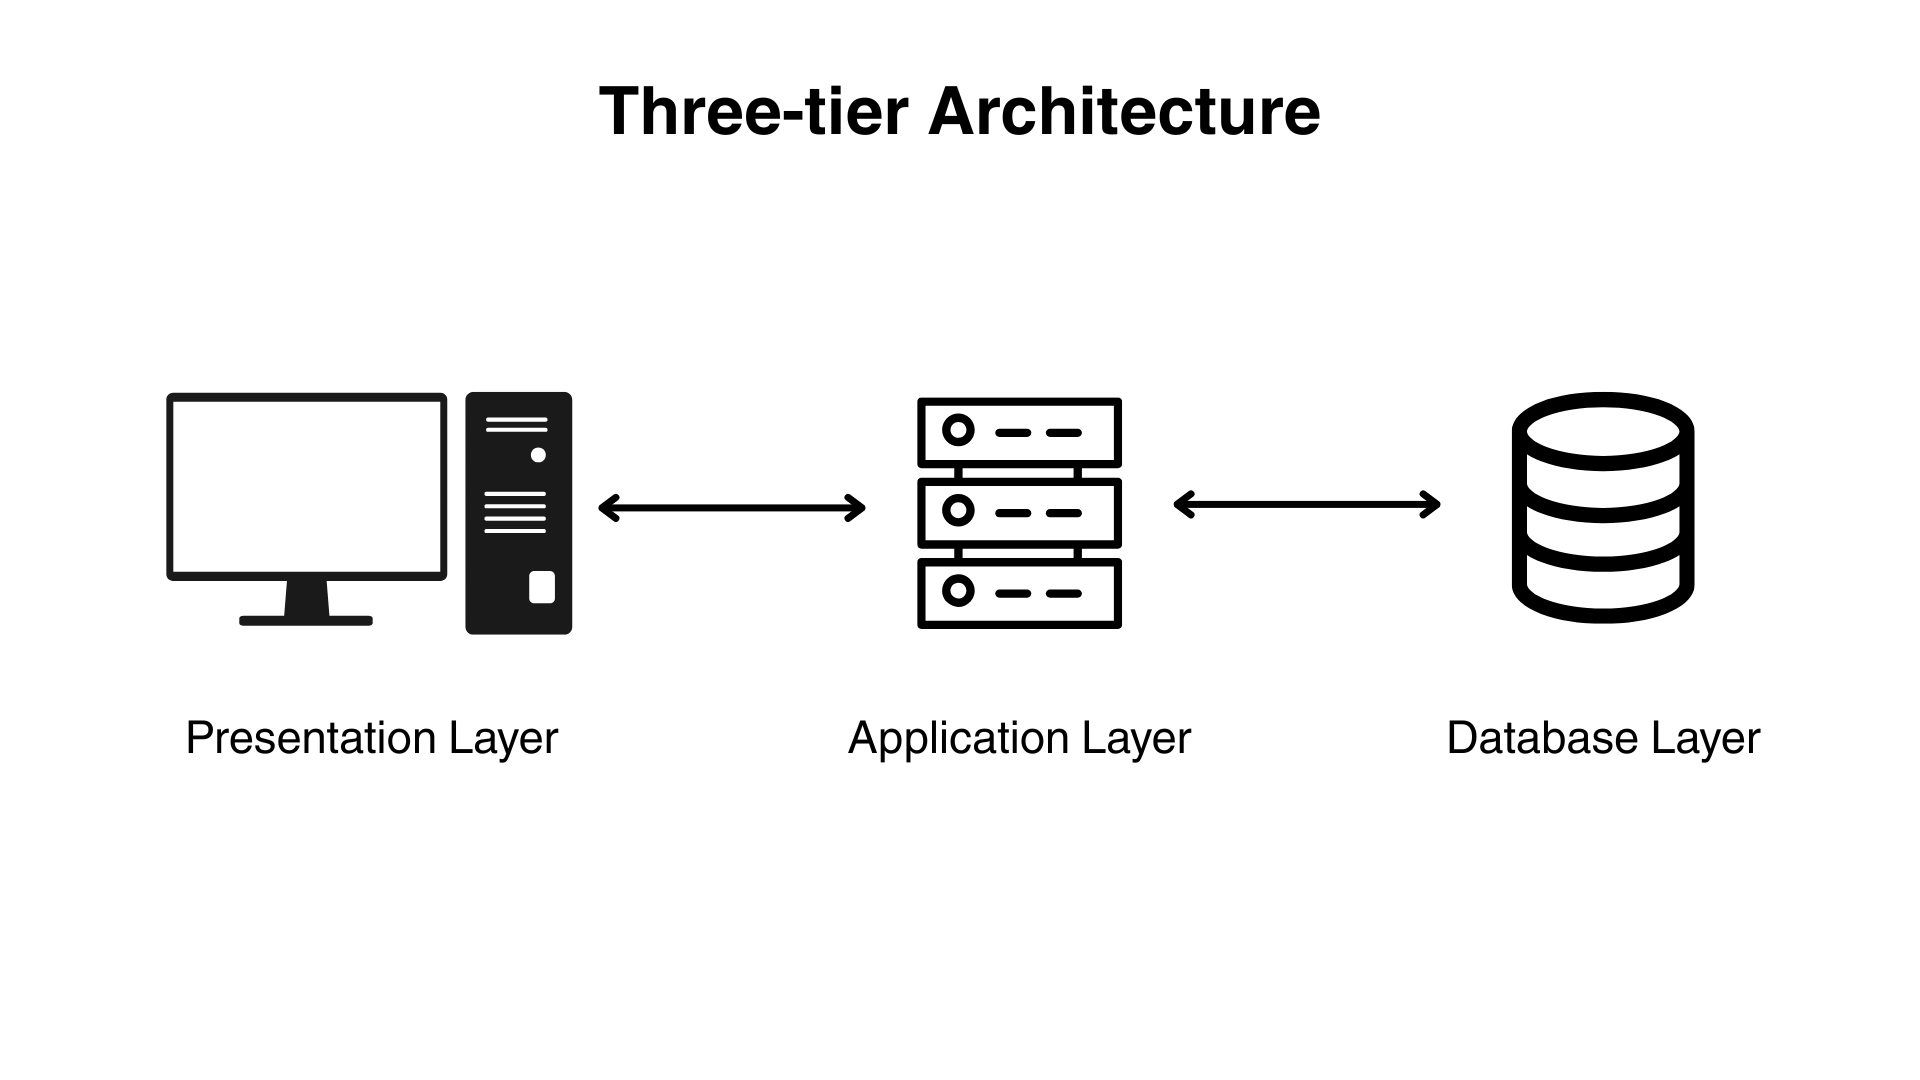
\includegraphics[width=0.85\textwidth]{Three_tier_architecture.png}
\caption{3-Tier System Architecture}
\label{fig:system-architecture}
\end{figure}

This chapter details the various technologies and resources that will be utilized in the development of Aphelion. 
The frontend, backend, database, framework, API, and other tools that are listed in this chapter were chosen after 
careful consideration, to serve as the infrastructure for the project – with explanation of the technology and reasoning 
regarding the advantages provided.

The project will be using a three-tier architecture, which includes the presentation layer, application layer, and database layer. This architecture allows us to focus on a specific concern without affecting the other layers, and it makes it easily scalable. The presentation layer is the interface that the users interact with. It handles user input and the display of the application. The application layer handles the business logic, which processes the user inputs from the presentation layer. This layer bridges the communication between the presentation layer to the database layer. The application layer handles the business logic, which processes the user inputs from the presentation layer. This layer bridges the communication between the presentation layer to the database layer, The database layer manages and stores the data used by the application. 

\section{Development Tools}

\subsection{Github}

\begin{figure}[h!]
\centering

\includegraphics[width=0.15\textwidth]{github.png}
\caption{Github Logo}
\label{fig:github-logo}
\end{figure}

GitHub enables collaboration remotely for development as repositories are stored in the cloud. It also allows version control, which helps with debugging the application.

\subsection{Lucidchart}

\begin{figure}[h!]
\centering

\includegraphics[width=0.15\textwidth]{lucidchart.png}
\caption{Lucidchart Logo}
\label{fig:lucidchart-logo}
\end{figure}

Lucidchart is used as a diagramming tool for visualizing theoretical system components such as the database and program flow.

\section{Technologies Used}

\subsection{React}

\begin{figure}[h!]
\centering

\includegraphics[width=0.15\textwidth]{react.png}
\caption{React Logo}
\label{fig:react-logo}
\end{figure}

React is a popular JavaScript-based frontend library with a notable focus on dynamic and responsive UI. It features reusable components which allows rapid construction of various interfaces, that of which the project heavily relies on, from the dialogue, text boxes, menus, minigames, and other forms of UI.

\subsection{Tailwind CSS}

\begin{figure}[h!]
\centering

\includegraphics[width=0.15\textwidth]{tailwind.png}
\caption{Tailwind CSS Logo}
\label{fig:tailwind-logo}
\end{figure}

Tailwind CSS offers a sleek and modern styling template framework that is wholly compatible with React. Tailwind’s utility classes allow for rapid prototyping and construction of user interfaces. Additionally, the responsive design allows UI elements to gracefully adapt to differing web browsers and hardware.

\subsection{PixiJS}

\begin{figure}[h!]
\centering

\includegraphics[width=0.15\textwidth]{pixijs.png}
\caption{PixiJS Logo}
\label{fig:pixijs-logo}
\end{figure}

PixiJS is a 2D WebGL render for web games. It handles sprite manipulation, animation, and interaction, which will be used for rendering the overall star map – the stars, planets, and other celestial bodies – in beautiful detail.

\subsection{Django}

\begin{figure}[h!]
\centering

\includegraphics[width=0.15\textwidth]{django.png}
\caption{Django Logo}
\label{fig:django-logo}
\end{figure}

Django is a Python-based web backend framework that will be the premier server-side tool for Aphelion, due to its generous features. Notably, Django’s Object-Relational Mapper synergizes well with PostgreSQL, streamlining the complex relationships between data, such as the Stars, Sectors, User Progress, and Sector Progress. Additionally, security features are provided out of the box. Django protects the system from SQL injection, Cross-Site Scripting, and CSRF attacks by default. Despite being more complicated and having more overhead than Express.js, we believe that utilizing Django for the backend is the more beneficial choice.

\subsection{PostgreSQL}

\begin{figure}[h!]
\centering

\includegraphics[width=0.15\textwidth]{postgresql.png}
\caption{PostgreSQL Logo}
\label{fig:postgresql-logo}
\end{figure}

PostgreSQL is an open-source relational database system, boasting robust and reliable performance. This database was chosen because of its integration with Django.

\subsection{HYG Database}

HYG Database is a compilation of 120,000 star data which will be used as the basis for accurate sector representation, ensuring a good educational value when students are engaging with the system.
%%%%%%%%%%%%%%%%%%%%%%%%%%%%%%%%%%%%%%%%%%%%%%%%%%%%%%%%%%%%%%%%%%%%%%%%%%%
\chapter{Methodology}
%%%%%%%%%%%%%%%%%%%%%%%%%%%%%%%%%%%%%%%%%%%%%%%%%%%%%%%%%%%%%%%%%%%%%%%%%%%

The Aphelion project will be developed using the Agile methodology, under the Kanban framework. The Agile methodology was chosen because of its flexible and iterative process, which provides numerous benefits in efficiently managing development time.  By dividing the work needed to be done, we can prioritize the most pressing aspects of the project to develop, and have a clear idea of the progress being made. Additionally, Kanban was chosen as the Agile framework because of its continuous workload style. The swimlanes provide a clear visual representation of progress – enabling to see what modules of the project are being worked on, and what priorities must be managed.

\begin{figure}[h!]
\centering
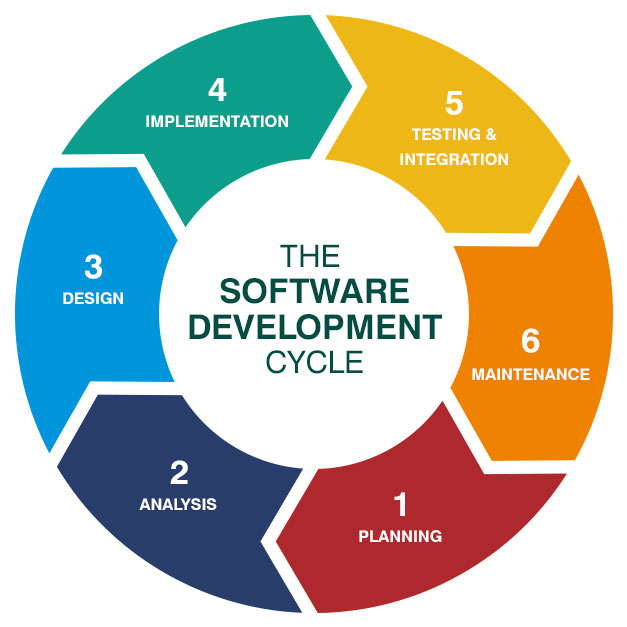
\includegraphics[width=0.15\textwidth]{agile.png}
\caption{Agile SDLC Model}
\label{fig:agile-sdlc}
\end{figure}

\begin{figure}[h!]
\centering
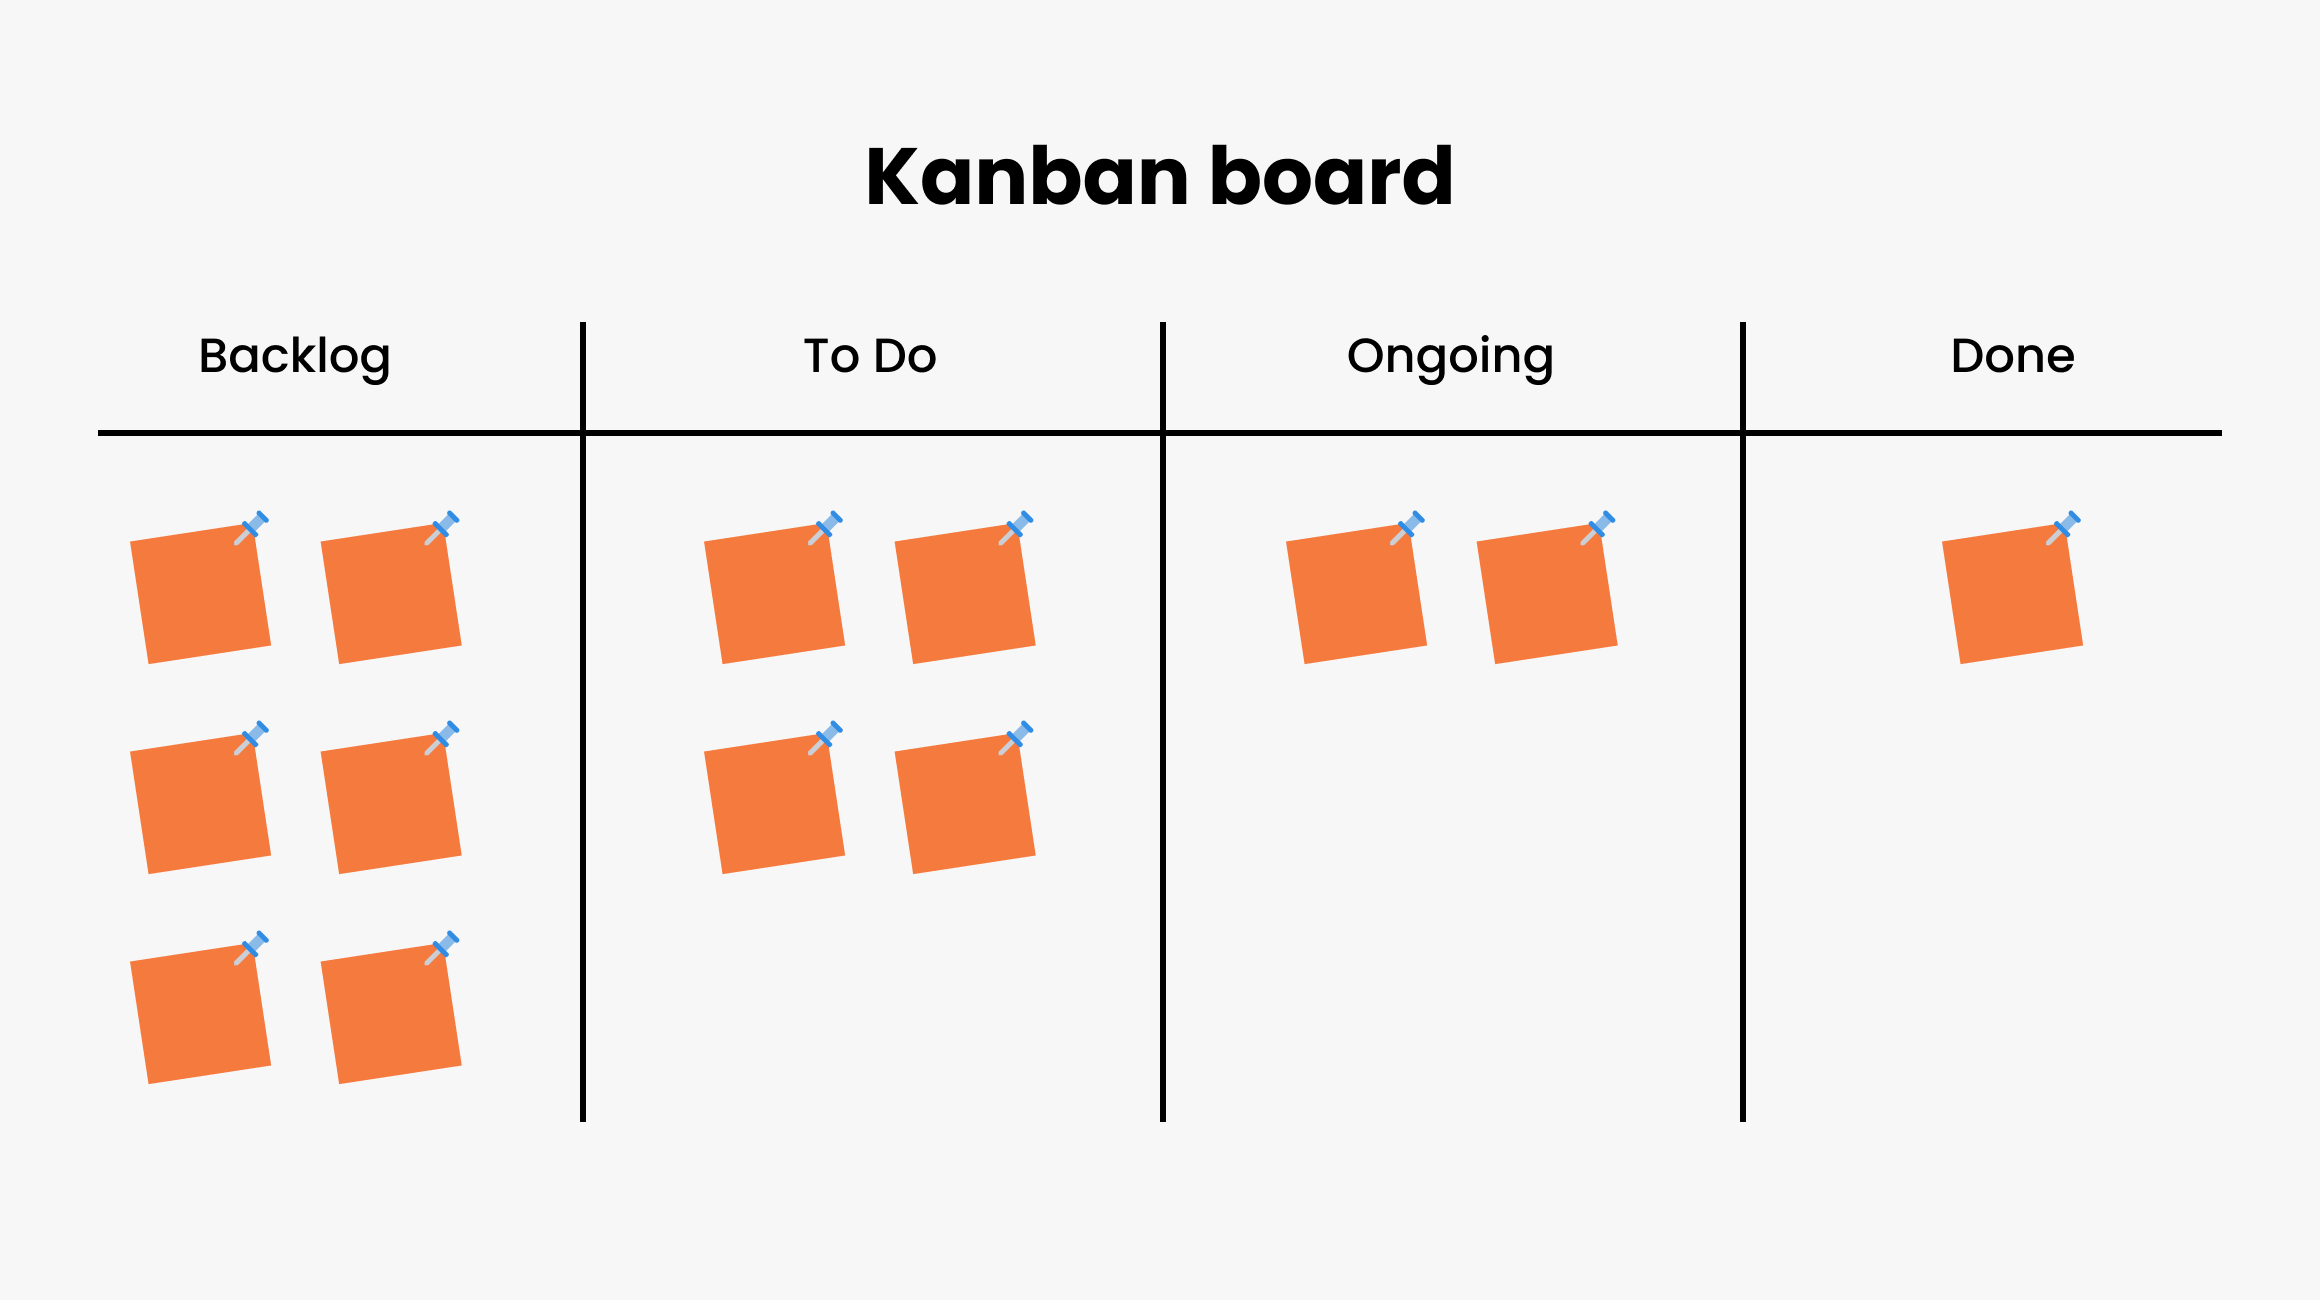
\includegraphics[width=0.15\textwidth]{kanban.png}
\caption{Kanban Board}
\label{fig:kanban-board}
\end{figure}

\section{Methodology Specification}

\subsection{Product Backlog List}

\textbf{User Story 1: Registration and Authentication}

As a user, I want to create an account and log in to access the program.

Functional Requirements:
\begin{itemize}
\item Account creation that requires a username, email, and password.
\item Password recovery using email.  
\item Login with a username and password.
\item Account deletion.
\end{itemize}

\textbf{User Story 2: Tutorial}

As a user, I want a short and simple tutorial that explains the game mechanics just enough for me to get a basic idea on what to do.

Functional Requirements:
\begin{itemize}
\item A short tutorial that explains how to:
\begin{itemize}
\item Choose a sector.
\item View stars on the star map.
\item Participate in ongoing exploration missions.
\item Complete minigames.
\end{itemize}
\end{itemize}

\textbf{User Story 3: Sector Selection}

As a user, I want to browse a list of servers that are exploring different star sectors, be able to see the progress of exploration for each sector, and to join the sector of my choosing.

Functional Requirements:
\begin{itemize}
\item A list of servers that users can join.
\item Shows the stars available and fully explored stars and number of users present.
\end{itemize}

\textbf{User Story 4: Star Exploration}

As a user, I want to see the map of stars in the sector that I joined and to pick unlocked stars to play the minigames and help with the exploration effort.

Functional Requirements:
\begin{itemize}
\item A star map that connects all the stars in a sector together.
\item Each star in the map exists in the HYG Database.
\item Star color and size are accurate to the corresponding database entry.
\item Visual elements indicating if a star is unexplored, fully explored, or has an ongoing exploration mission.
\end{itemize}

\textbf{User Story 5: Minigames}

As a user, I want to be presented with a random selection of minigames called “missions” to aid in the stellar exploration effort, with the minigames being thematic to astronomy and space exploration.

Functional Requirements:
\begin{itemize}
\item A number of educational minigames based on astronomy concepts.
\end{itemize}

\textbf{User Story 6: Celestial Body Description}

As a user, I want to view descriptions of the star being explored, as well as the planets orbiting it.

Functional Requirements:
\begin{itemize}
\item Text descriptions for every celestial body in a star system.
\end{itemize}

\textbf{User Story 7: Levelling System}

As a user, I want to accumulate experience points whenever I complete minigames for the exploration missions of a star, with rewards being unlocked as I level up.

Functional Requirements:
\begin{itemize}
\item Level system for players based on minigames completed.
\item Rewards for higher levels.
\end{itemize}

\textbf{User Story 8: Account Information and Statistics}

As a user, I want to view my public account information such as my username and profile picture, as well as my private information such as my email. I also want to view my lifetime statistics for the game.

Functional Requirements:
\begin{itemize}
\item Profile page with views for public and private information.
\item The available information can be edited.
\item The profile page has a separate view for user statistics.
\end{itemize}

\textbf{User Story 9: Achievements and Badges}

As a user, I want to unlock achievements when I play the game in certain ways, and display them in my profile page as badges.

Functional Requirements:
\begin{itemize}
\item Achievements that trigger during specific actions, example:
\begin{itemize}
\item Complete an exploration minigame for 5 days.
\item Reach level 20.
\item Be the first to start an exploration mission.
\end{itemize}
Badges that are acquired from achievements that can be displayed on the profile page.
\end{itemize}

\textbf{User Story 10: Gameplay Collaboration}

As a user, I want to send friend requests to other users, and be able to invite them in ongoing exploration missions.

Functional Requirements:
\begin{itemize}
\item An option to send friend requests to other users.
\item A user can send invites to friends that will lead to the same sector and star that the sender is in.
\end{itemize}

\textbf{User Story 11: Admin Privileges}

As a super user, I want to start star sectors and generate the stars based on proximity to create a coherent map. I also want to be able to edit descriptions of celestial bodies.

Functional Requirements:
\begin{itemize}
\item Generate sectors that users can join in.
\item Edit text descriptions for celestial bodies anytime.
\end{itemize}

Non-functional Requirements:
\begin{itemize}
\item Performance: Aphelion should run on weaker hardware without much difficulties, should have responsive buttons, and quick loading times – descriptions for celestial bodies must show near instantaneously.
\item Reliability: Redundant servers must be present to ensure that users can continue playing through technical issues.
\item Usability: The UI/UX must be simple and intuitive, requiring minimal tutorial to be usable.
\item Scalability: Aphelion must have a robust system that can handle the stress from increasing players and active servers.
\item Compliance on Regulations: Aphelion must abide by the law regarding user consent and privacy.
\end{itemize}

\subsection{Agile Workload Management}

\textbf{Sprint Planning}

Aphelion will be developed in spans of 1 week called “sprints”, according to the Agile methodology. During each sprint, one or more related tasks in the kanban will be moved into the “ongoing” swimlane and will be worked upon.

\textbf{Daily Stand-up Meeting}

Every day, the development team will communicate for no more than 5 minutes in order to give a short overview of tasks done, and the state of the project as a whole. Ideally, this meeting will be done face-to-face while standing up, emphasizing the namesake. Online meetings are also considered.

\textbf{Backlog Review}

At the end of a sprint, the development team will consider the next set of user stories to be completed for the following sprint.

\section{Systems Analysis}

\subsection{Application Modules}

\textbf{Account Creation/Login}

The account creation/login module facilitates the creation and deletion of user accounts, as well as verification during sessions. A button in the landing page prompts the user to login or sign up, with the latter requiring:

\begin{itemize}
\item Username - A maximum of 20 characters, no spaces.
\item Email Address - Must be valid, and the user must verify the address.
\item Password - A minimum length of 8 characters must be met, otherwise all types of password strength is allowed. A bar displaying the password strength is shown.
\end{itemize}

Once the user creates an account, they can login using the username and password.

\textbf{Celestial Data Provider}

This module communicates with the Nasa Exoplanet API and HYG Database and loads the relevant, scientifically accurate data when generating sectors.

\textbf{Star Map}

The star map module serves as the visual representation of a sector. A facilitator generates the sector, which automatically picks the collection of stars based on relative range. Students can then join sectors and participate in exploration missions.

\textbf{Missions}

The mission module handles the selection of minigames that the user will play to complete the exploration effort for a star. It tracks the mission details and progress, and rewards players with badges upon completion.

\textbf{Profile}

The profile module is connected to an account, and updates accordingly as the user interacts with the program.

\section{System Design}

\subsection{Use Case Diagram}

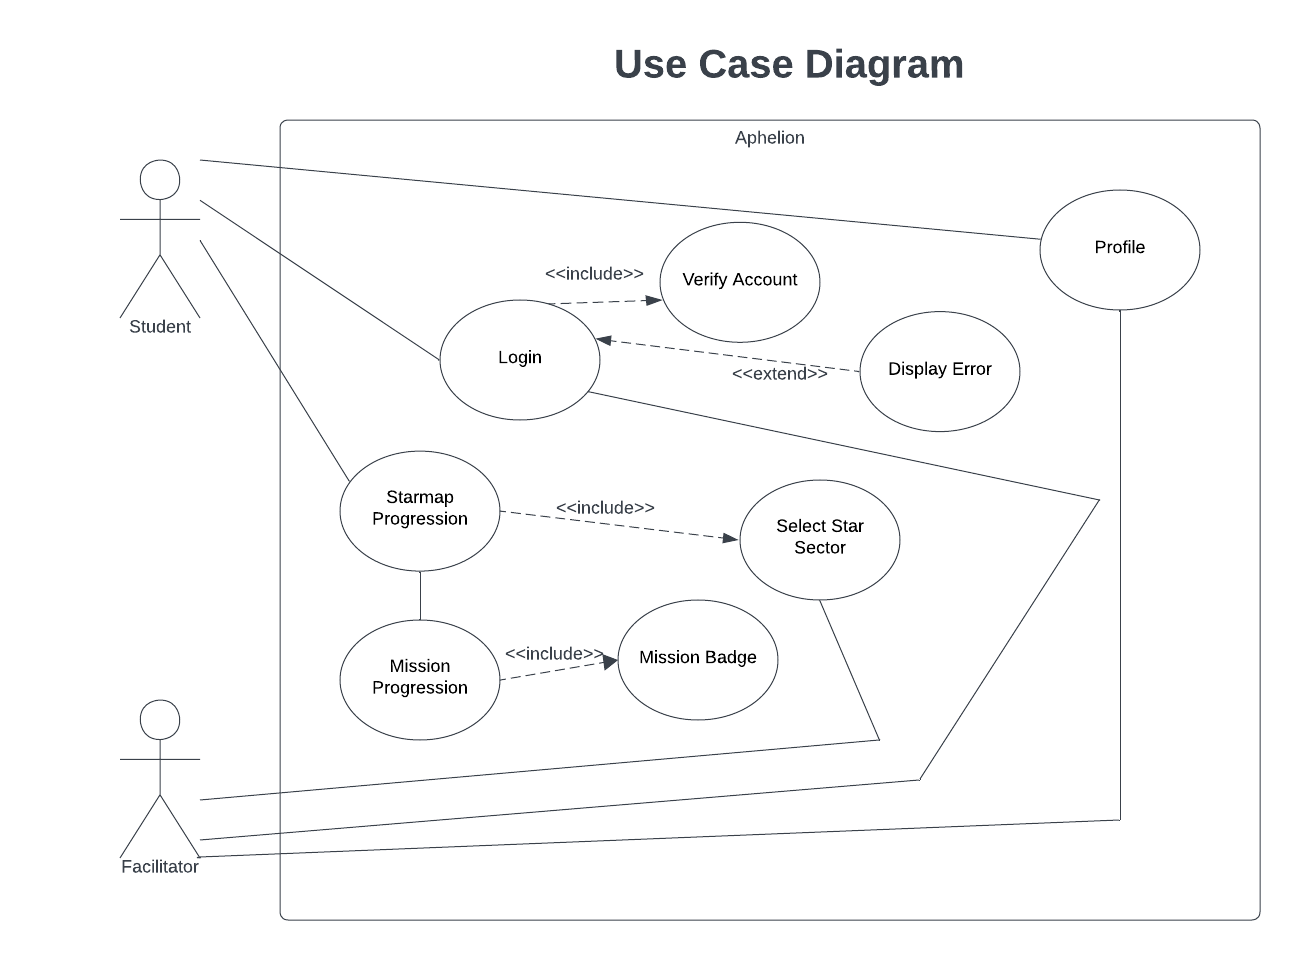
\includegraphics[width=0.95\textwidth]{Use_Case.png}
\begin{figure}[h!]
\centering
\caption{Use Case Diagram}
\label{fig:use-case}
\end{figure}

\FloatBarrier
\subsection{Context Diagram}

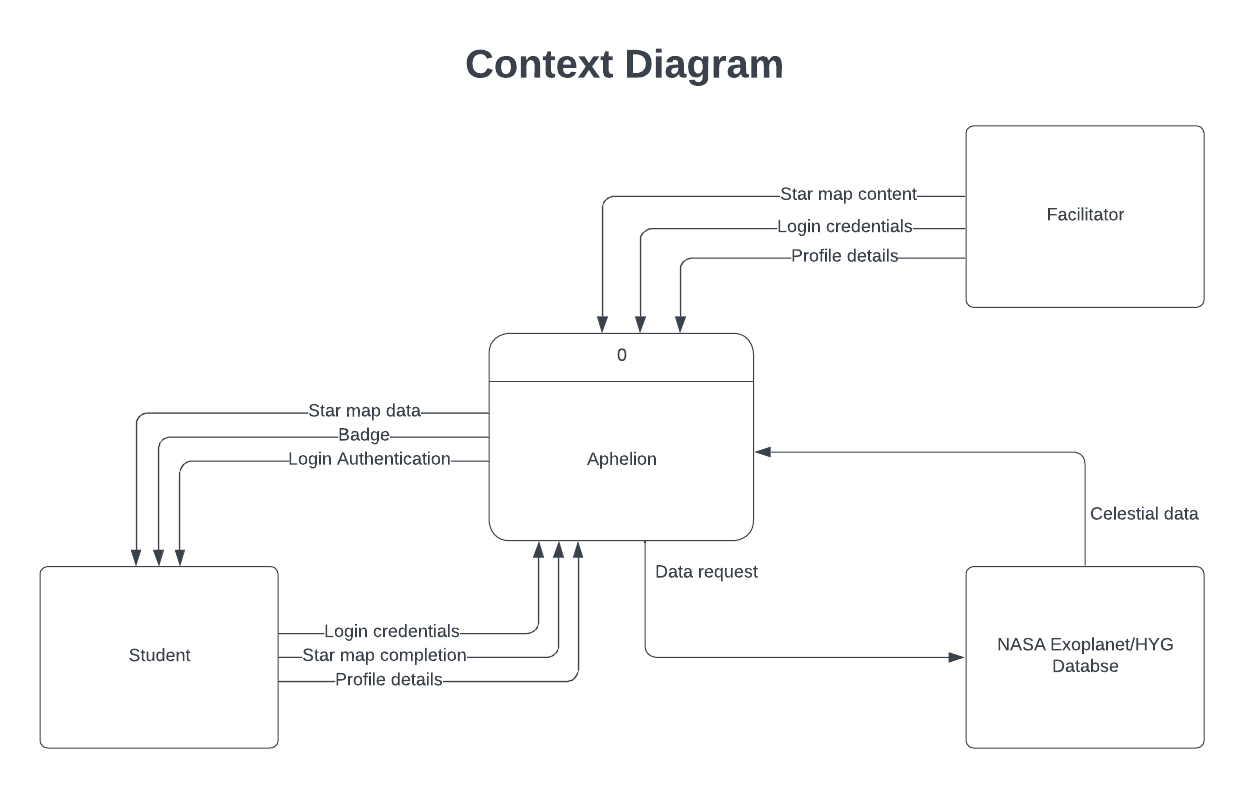
\includegraphics[width=0.95\textwidth]{Context_Diagram.png}
\begin{figure}[h!]
\centering
\caption{Context Diagram}
\label{fig:context-diagram}
\end{figure}

\FloatBarrier
\subsection{Data Flow Diagram}

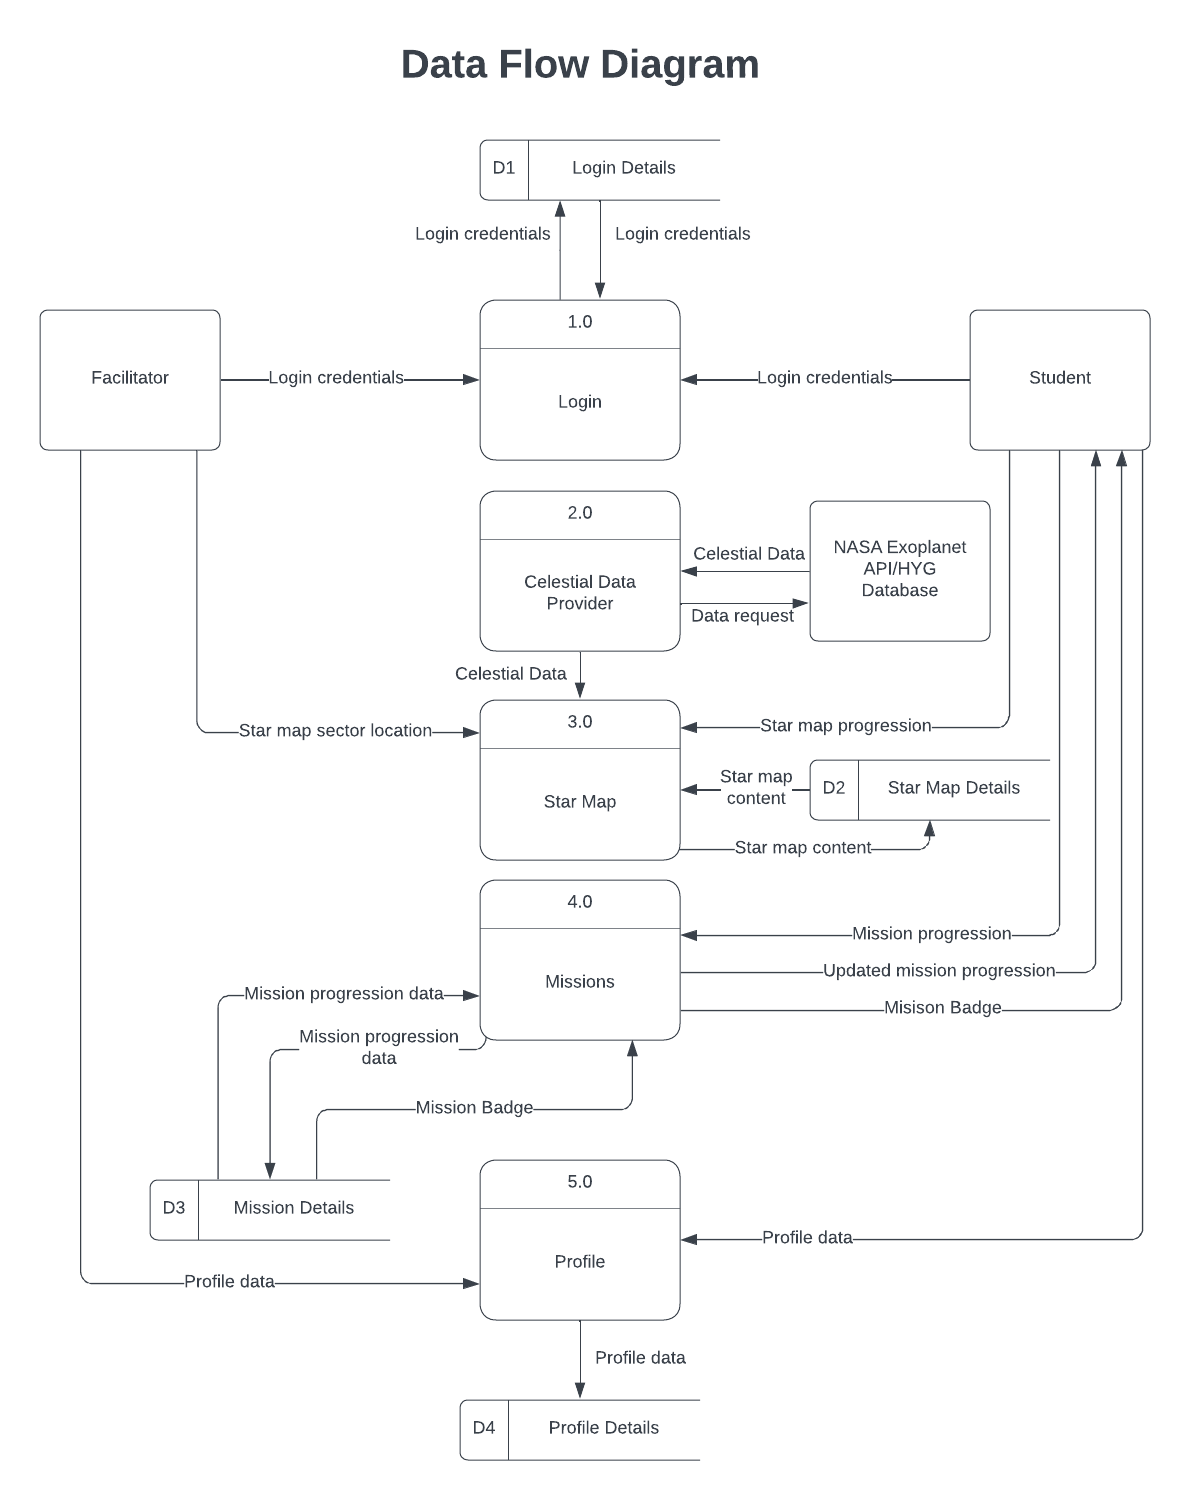
\includegraphics[width=0.95\textwidth]{Data_Flow_Diagram.png}
\begin{figure}[h!]
\centering
\caption{Data Flow Diagram}
\label{fig:data-flow-diagram}
\end{figure}

\FloatBarrier
\subsection{Level 2 Data Flow Diagram}

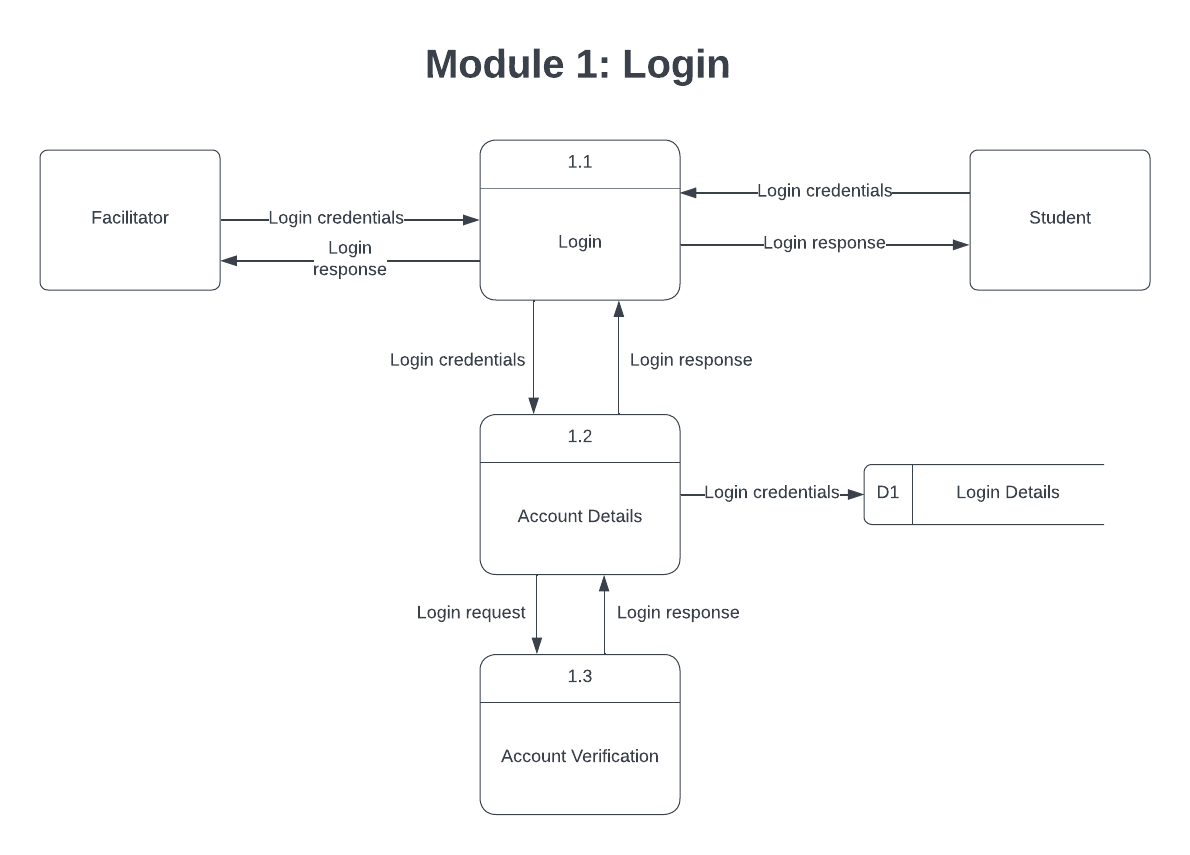
\includegraphics[width=0.95\textwidth]{Module_1.png}
\begin{figure}[h!]
\centering
\caption{Module 1}
\label{fig:module-1}
\end{figure}

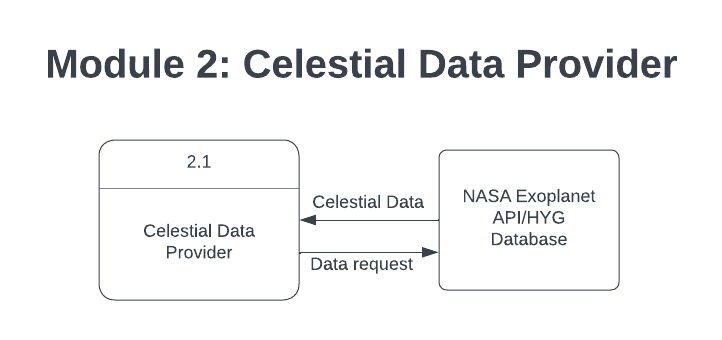
\includegraphics[width=0.95\textwidth]{Module_2.png}
\begin{figure}[h!]
\centering
\caption{Module 2}
\label{fig:module-2}
\end{figure}

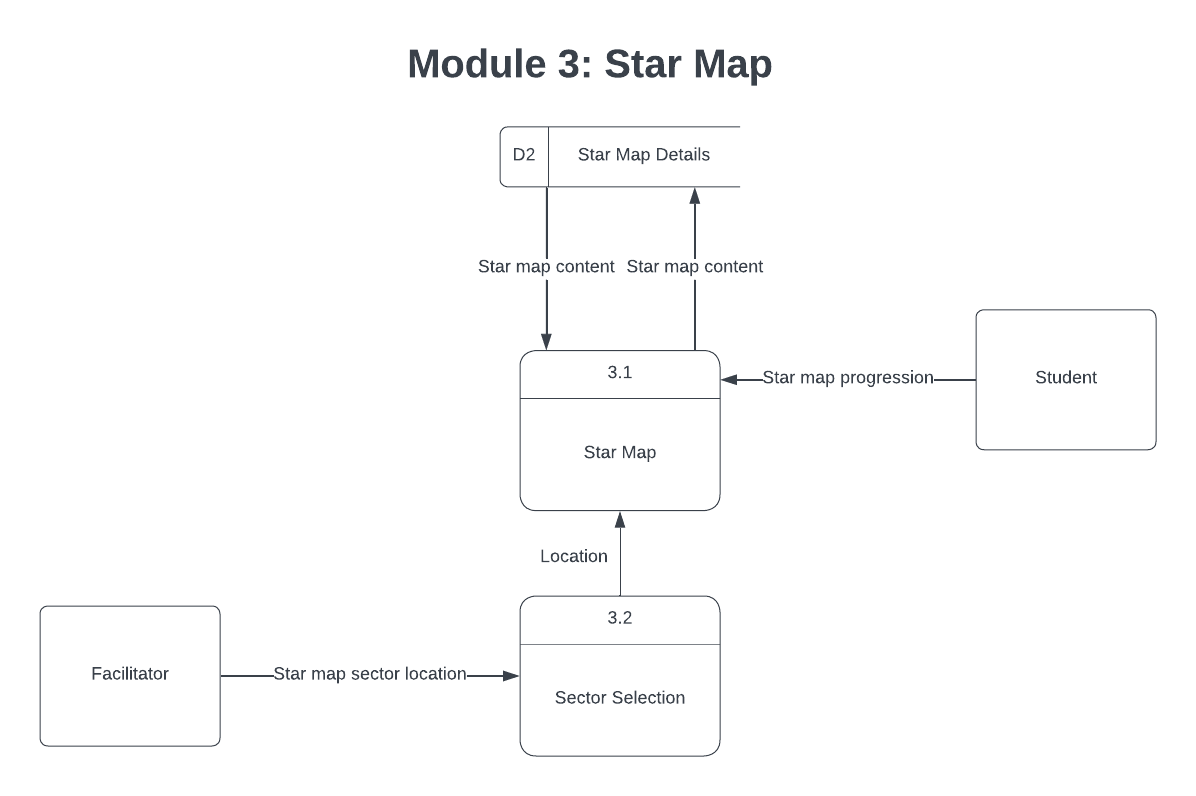
\includegraphics[width=0.95\textwidth]{Module_3.png}
\begin{figure}[h!]
\centering
\caption{Module 3}
\label{fig:module-3}
\end{figure}

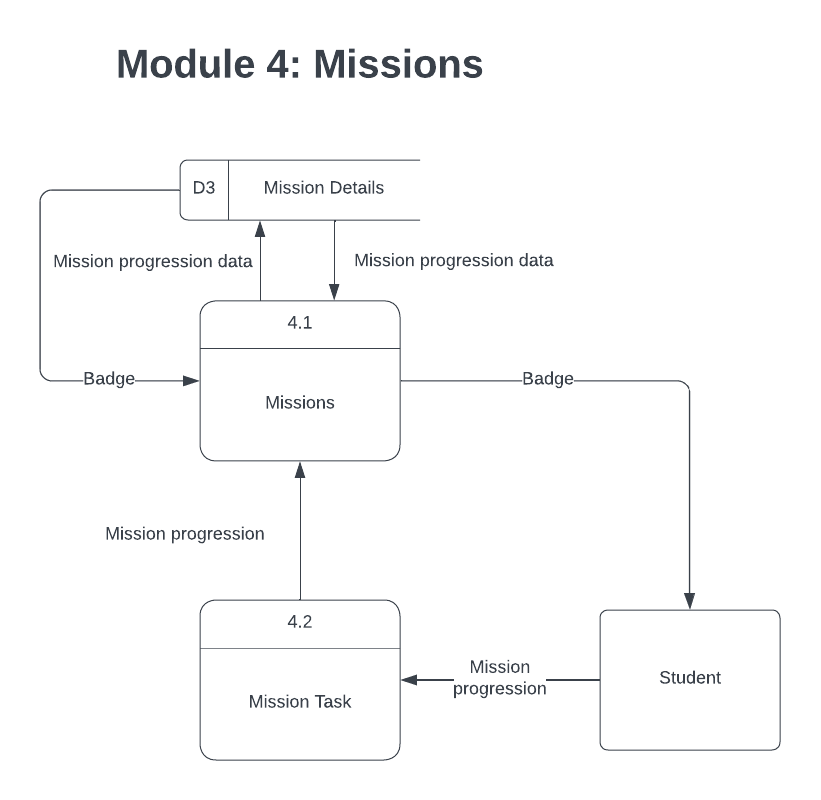
\includegraphics[width=0.95\textwidth]{Module_4.png}
\begin{figure}[h!]
\centering
\caption{Module 4}
\label{fig:module-4}
\end{figure}

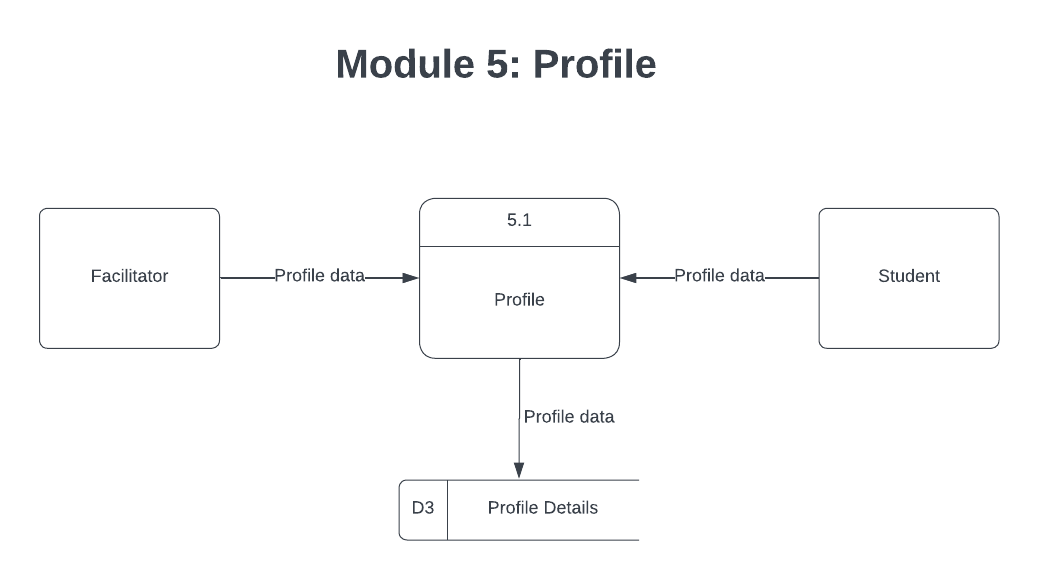
\includegraphics[width=0.95\textwidth]{Module_5.png}
\begin{figure}[h!]
\centering
\caption{Module 5}
\label{fig:module-5}
\end{figure}

\FloatBarrier
\subsection{Process Flow Diagram}

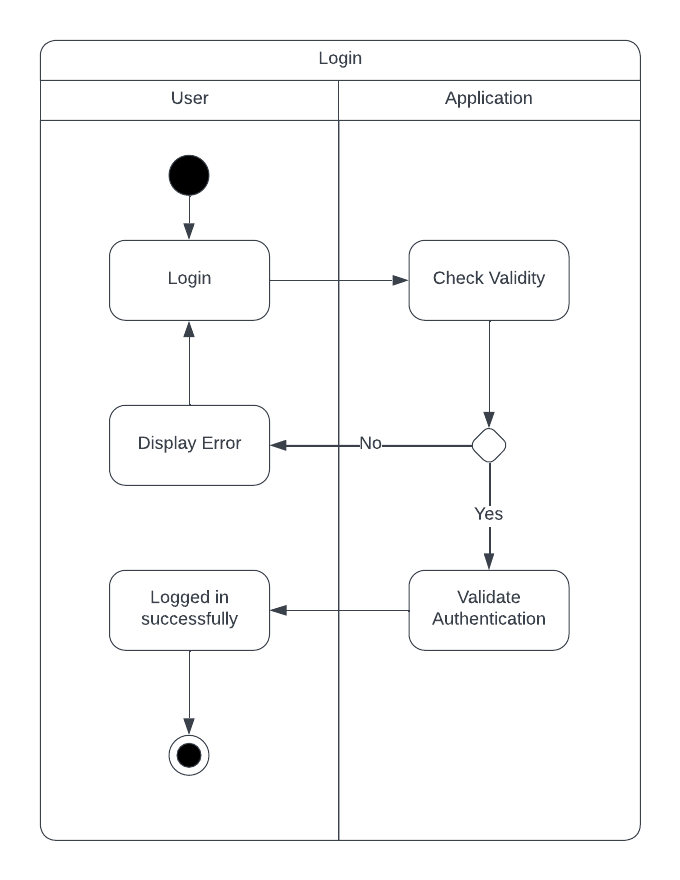
\includegraphics[width=0.95\textwidth]{Process_Flow_ Login.png}
\begin{figure}[h!]
\centering
\caption{Process Flow Diagram}
\label{fig:process-flow-login}
\end{figure}

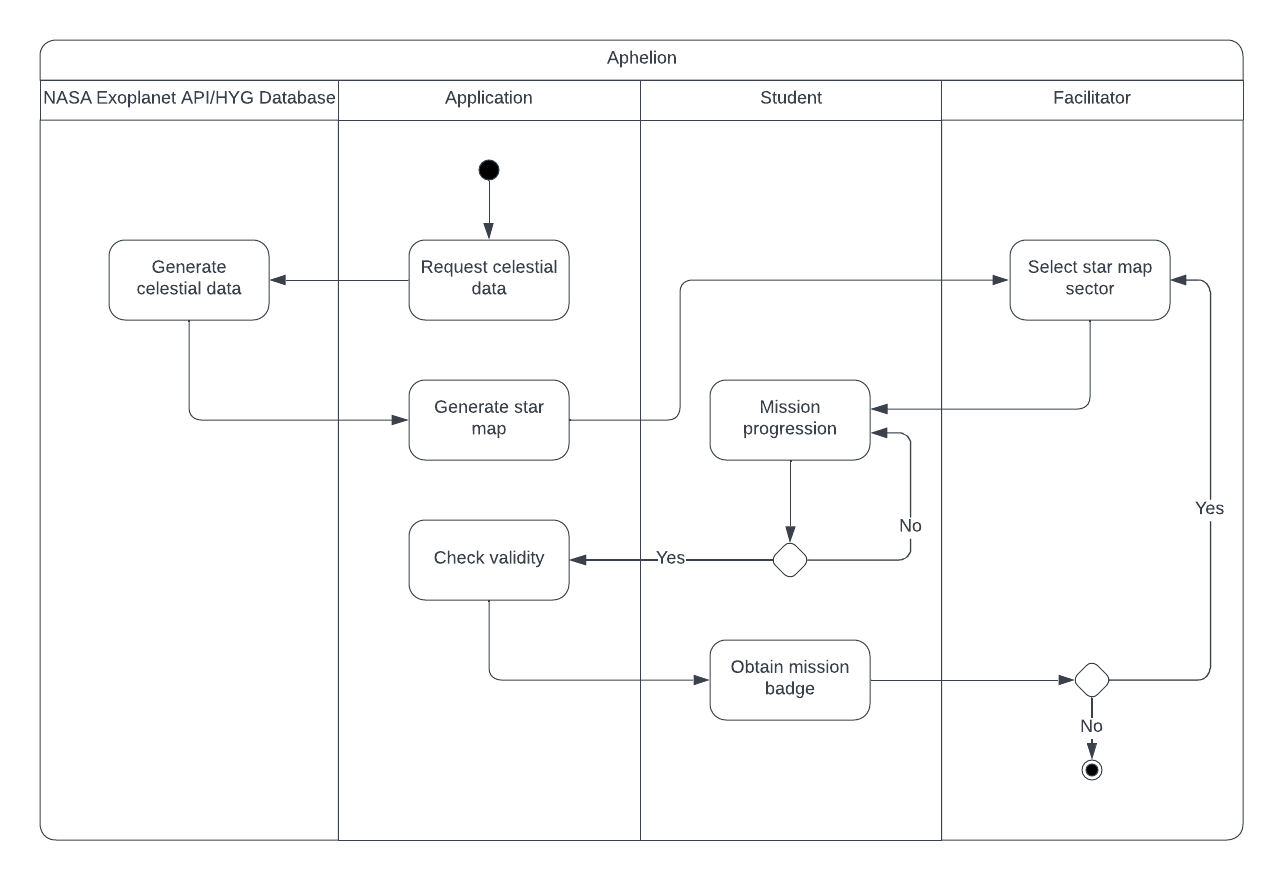
\includegraphics[width=0.95\textwidth]{Activity.png}
\begin{figure}[h!]
\centering
\caption{Activity Diagram}
\label{fig:process-flow-diagram}
\end{figure}

\FloatBarrier
\subsection{Entity Relationship Diagram}

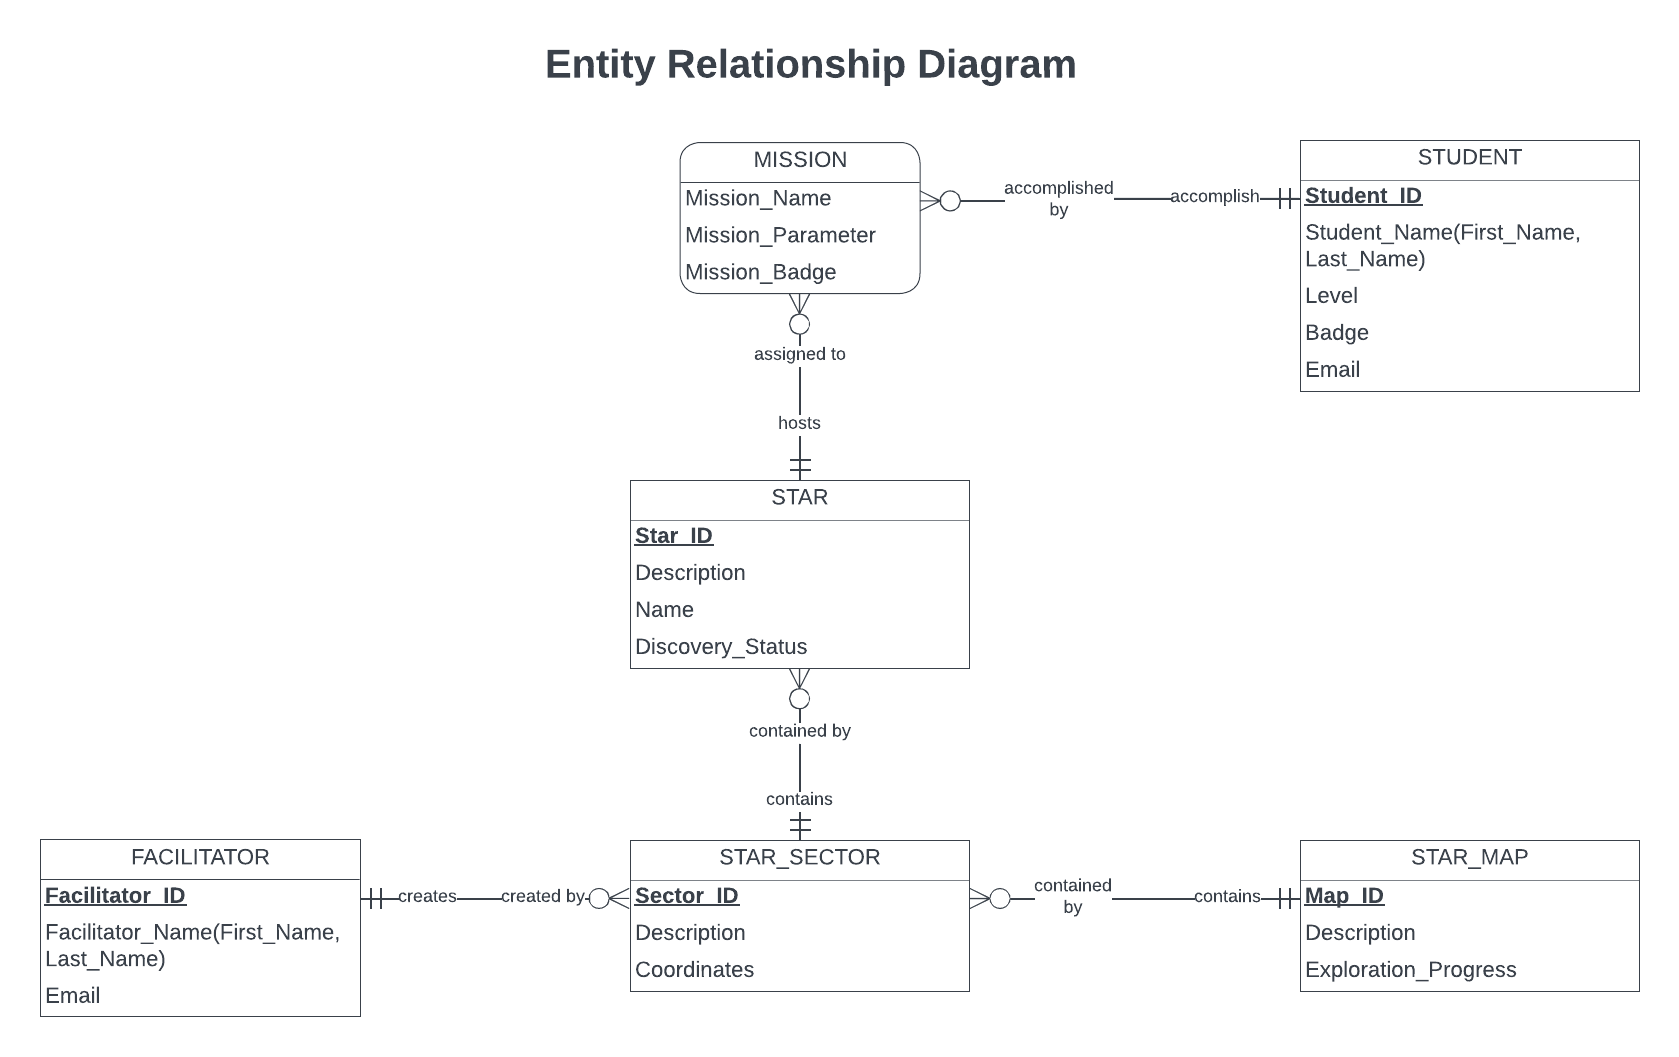
\includegraphics[width=0.95\textwidth]{ERD.png}
\begin{figure}[h!]
\centering
\caption{Entity Relationship Diagram}
\label{fig:erd}
\end{figure}
%\include{chapters/results}
%\include{chapters/recommendations}
% \include{chapters/conclusion} may also be used

\appendix
%    \include{appendices/evaltool}
%    \include{appendices/reports}
%    \include{appendices/io}
%    \include{appendices/code}
 %   \include{appendices/usersguide}

\nocite{*}
\bibliographystyle{siam}
{
\singlespace
\bibliography{references}
}

\begin{vita}

Harold James R Azur is BS Information Technology student of the Department of Computer Science at the Ateneo de Naga University.
\\
\\
Giankarlo F. Rivera is BS Information Technology student of the Department of Computer Science at the Ateneo de Naga University.

\end{vita}

\end{document}
